%%	This is file 'hackthefootline-doc.tex', Version 2018-01-28
%%	Copyright 2017-18 Sebastian Friedl <sfr682k@t-online.de>
%% 
%%	This work may be distributed and/or modified under the conditions of the LaTeX Project
%%	Public License, either version 1.3c of this license or (at your option) any later version.
%%	The latest version of this license is available at
%%		http://www.latex-project.org/lppl.txt
%%	and version 1.3c or later is part of all distributions of LaTeX version 2008-05-04 or later
%%
%%	This work has the LPPL maintenace status 'maintained'.
%%	The current maintainer of this work is Sebastian Friedl.
%%
%%	This work consists of the files hackthefootline.sty, hackthefootline-examples.tex and
%%	hackthefootline-doc.tex
%%
%%	-------------------------------------------------------------------------------------------
%%
%%	The hackthefootline package is a tool providing arbitrary footline selection and
%%	configuration for LaTeX beamer's standard themes (it may work with other themes as well)
%%
%%	-------------------------------------------------------------------------------------------
%%
%%	Please report bugs and other problems as well as suggestions for improvements
%%	to my email address (sfr682k@t-online.de).
%%
%%	-------------------------------------------------------------------------------------------
%%
%%	Acknowledgement:
%%	The basic layout of the two- and three-column footline is based on the original LaTeX
%%	beamer split and infolines outer themes written by Till Tantau.
%%
%%	-------------------------------------------------------------------------------------------

% !TeX spellcheck = en_GB

% !TeX document-id = {681db40e-7a84-4428-b4f4-84e230e3ba79}
% !TeX program=lualatex
% !TeX TXS-program:compile=txs:///lualatex/[--shell-escape]


\documentclass[11pt]{ltxdoc}

\usepackage[erewhon]{newtxmath}
\usepackage[no-math]{fontspec}
\usepackage{polyglossia}
\setdefaultlanguage{english}

\usepackage{csquotes}
\usepackage{hologo}
\usepackage[pdfborder={0 0 0}, unicode]{hyperref}
\usepackage[english]{selnolig}
\usepackage{tikz}

\newcommand{\DescribeOption}[3]{
  \DescribeMacro{#1}
  \begin{minipage}[t]{\textwidth}
    \textit{\textbf{#2}}\dotfill~\par
    \begingroup
    \vspace{0.5em}#3\par
    \endgroup
  \end{minipage}%
  \bigskip\medskip%
}


\parindent 0pt

\setmainfont{erewhon}
\setsansfont[Scale=MatchLowercase]{Source Sans Pro}
\setmonofont[Scale=MatchLowercase]{Hack}

\usepackage[left=4.50cm,right=2.75cm,top=3.25cm,bottom=2.75cm,nohead]{geometry}

\hyphenation{coun-ted}
\MakeShortVerb{"}


\title{The \texttt{\bfseries hackthefootline} package \\ {\large\url{https://github.com/SFr682k/hackthefootline}}}
\author{Sebastian Friedl \\ \href{mailto:sfr682k@t-online.de}{\ttfamily sfr682k@t-online.de}}
\date{2018/01/28}

\hypersetup{pdftitle={The hackthefootline package},pdfauthor={Sebastian Friedl}}

\begin{document}
	\maketitle
	\thispagestyle{empty}
	
	\begin{center} \itshape
		Dedicated to all the \LaTeX\ beamer users \dots
		
		\medskip
		\dots who load two different themes in the same presentation \\ or redefine commands to obtain the desired footline \dots
		
		\medskip
		\dots and the other guys just using "\setbeamertemplate"
	\end{center}
	
	\medskip
	\begin{abstract}
		\parindent0pt\noindent%
		\textbf{Arbitrary footline selection and configuration for \LaTeX\ \texttt{beamer}'s standard themes.} \\
		"hackthefootline" is a package taking over, defining and redefining different footlines, so they can be configured using key-value syntax.
		
		\smallskip
		The basic layout of the two- and three-column footline is based on the original \LaTeX\ beamer split and infolines outer themes written by Till Tantau.
	\end{abstract}
	
	
	\tableofcontents
	
	\clearpage
	
	
	
	\subsection*{Dependencies and other requirements}
	\addcontentsline{toc}{subsection}{Dependencies and other requirements}
	%
	\DescribeMacro{beamer}
	Since "hackthefootline" is designed to modify "beamer"'s footlines, it is incompatible to any other document class. Therefore, load this package only in "beamer" documents!
	
	\medskip
	\DescribeMacro{pgfkeys}
	"hackthefootline" heavily depends on the "pgfkeys" package for handling the whole key-value stuff.
	
	\bigskip
	Also, additional sophisticated features require the following packages:
	
	\medskip
	\DescribeMacro{appendixnumber-}\DescribeMacro{beamer}
	\textbf{Only required when using \texttt{beamer} version 3.48 and older.}
	This package is only required when using "beamer" version 3.48 or older. If you are using "beamer" version 3.49 or later\footnote{i. e. \TeX{}Live 2018 and later}, "hackthefootline" will rely on "beamer"'s internal appendix frame numbering mechanisms.
	
	\medskip
	\DescribeMacro{etoolbox}
	Provides access on \hologo{eTeX} primitives
	
	\medskip
	\DescribeMacro{calc}
	Required for basic calculations

	\medskip
	\DescribeMacro{numprint}
	Prints out numbers, counters and lengths
	
	\bigskip
	However, the four latter dependencies can be removed by using some package options. See section \ref{behavioropts} for further details.
	
	
	\subsection*{Notice: Behavior inside the presentation's appendix}
	\addcontentsline{toc}{subsection}{Notice: Behavior inside the presentation's appendix}
	By default, appendix frames are \emph{not} counted into the total number of frames when using "hackthefootline". Appendix frame numbers will be counted from 1 when using fraction frame numbers. \\
	Also, frame numbers won't be displayed on footlines inside the appendix until this is changed using the means of the "\htfconfig" command.
	
	\medskip
	This behavior can be suppressed by passing the "countappendixframes" option.
	
	
	\subsection*{License}
	\addcontentsline{toc}{subsection}{License}
	\textcopyright\ 2017-18 Sebastian Friedl
	
	\smallskip
	This work may be distributed and/or modified under the conditions of the \LaTeX\ Project Public License, either version 1.3c of this license or (at your option) any later version.
	
	\smallskip
	The latest version of this license is available at \url{http://www.latex-project.org/lppl.txt} and version 1.3c or later is part of all distributions of \LaTeX\ version 2008-05-04 or later.
	
	\smallskip
	This work has the LPPL maintenace status \enquote*{maintained}. The current maintainer of this work is Sebastian Friedl. \\
	This work consists of the following files:
	\begin{itemize} \itemsep 0pt
		\item "hackthefootline.sty"
		\item "hackthefootline-examples.tex" and
		\item "hackthefootline-doc.tex"
	\end{itemize}
	
	
	
	\clearpage



	% DOCUMENTATION PART ------------------------------------------------------------------------------------------------------------------------

	\section{Using the package}
	The "\usepackage[<Options>]{hackthefootline}" command loads the package\footnote{To do so, the package has to be installed in a location where \LaTeX\ is able to find it}. A list of all available options can be found in section \ref{packageoptions}.
	
	\medskip
	\textbf{Important note:} You \emph{have} to pass the \emph{footline's number of columns} as an option to the package (available: "onecol", "twocols" or "threecols"). If you don't do so, the footline gets removed completely. \\
	See section \ref{examples-setup} for some examples.
	
	
	
	\section{Package options} \label{packageoptions}
	\subsection{Options influencing the footline's configuration}
	These options determine the number of columns being used for the footline. \\
	You \emph{have} to pass one of these options when loading "hackthefootline"; otherwise the footline will be removed completely.
	
	\medskip
	\DescribeMacro{onecol}
	The \enquote{initial footline hack} produces a one--column footline
	
	\medskip
	\DescribeMacro{twocols}
	The \enquote{initial footline hack} produces a two--column footline
	
	\medskip
	\DescribeMacro{threecols}
	The \enquote{initial footline hack} produces a three--column footline
	
	\subsection{Options influencing the package's behavior} \label{behavioropts}
	These options can be passed to disable additional features and remove dependencies on other packages.
	
	\medskip
	\DescribeMacro{countappendix-}\DescribeMacro{frames}
	If the "countappendixframes" option is passed to the package, appendix frames are counted into the total number of frames. \\
	\textit{Removes the following dependencies:} "appendixnumberbeamer", "etoolbox"
	
	\medskip
	\DescribeMacro{nofun}
	Doesn't support frame numbers being shown as \enquote{percent of presentation} \\
	\textit{Removes the following dependencies:} "calc", "numprint"



	\section{Configuring the footline}
	The internal mechanisms of "hackthefootline" are using templates for displaying the provided information.
	Each template is available in different styles, which can be switched using the provided key value syntax:
	
	\medskip
	\DescribeMacro{\htfconfig}
	Use "\htfconfig{key1=value1, key2=value2, …}" to modify the current configuration of the footline. Changes apply instantly. \\
	See section \ref{examples-switchtemplates} for examples.
	
	\bigskip
	All available keys and values are listed below being depicted as follows:
	
	\medskip
	\DescribeOption{key}{possible values}{Description of the values' effects}
	
	\medskip
	\textbf{Annotations:}
	\begin{itemize}
		\item
			The default values of the keys depend on the number of columns chosen when loading the package. See section \ref{defaultconfig} for further details.
		\item
			\textit{Templates not visible} in the default configuration have been hidden by setting the value of the according key to "none". Apply another value to this key and the template will show up. \\
			\textit{Templates visible} in the default configuration can be hidden by setting the value of the according key to "none" (there's only one exception: "atsep"). \\
			See section \ref{examples-switchtemplates} for examples.
	\end{itemize}
	
	\bigskip
	\DescribeOption{cols}{one, two, three, none}{%
		The number of colums used for the footline:
		\begin{description}\itemsep0pt
			\item[one]
				Use a footline consisting of a single column
			\item[two]
				Use a footline consisting of two columns
			\item[three]
				Use a footline consisting of three columns
			\item[none]
				Remove the footline completely
		\end{description}
		
		Although the "cols" key's value changes, the other keys' values stay the same. \textbf{If you change the number of columns of a footline, the other keys should be adjusted as well.}
		
		\medskip
		\emph{Warning:} Changing this key's value too often might distract your audience.
	}
	
	\DescribeOption{title}{short, long, none}{%
		Sets the title type displayed in the footline:
		\begin{description}\itemsep0pt
			\item[short]
				Show the short title given in the square braces of the \texttt{\textbackslash title} command. \\
				When no short title is given, the long title will be used.
			\item[long]
				Show the long title given in the curly braces of the \texttt{\textbackslash title} command.
			\item[none]
				Don't show any title inside the footline
		\end{description}}
	
	\DescribeOption{authinst}{onlyauthor, onlyinst, instpths, authpths, both, none}{%
		Influences the way author and institute are displayed:
		\begin{description}\itemsep0pt
			\item[onlyauthor]
				Show only the author's name
			\item[onlyinst]
				Show only the institute's name
			\item[instpths]
				Show both, author and institute, but put the institute into parentheses
			\item[authpths]
				Show both, author and institute, but put the author into parentheses
			\item[both]
				Show both and separate them using a comma
			\item[none]
				Show neither author, nor institute
		\end{description}
		All templates use the values specified for short author / short institute.
	}
	
	\DescribeOption{date}{short, long, none}{%
		The date displayed in the footline:
		\begin{description}\itemsep0pt
			\item[short]
				Show the short date
			\item[long]
				Show the long date
			\item[none]
				Do not show any date
		\end{description}}
	
	\DescribeOption{framenrs}{counter, fraction, percent, none}{%
		Controls the type of frame number shown in the footline:
		\begin{description}\itemsep0pt
			\item[counter]
				Only show the number of the current frame
			\item[fraction]
				Show the number of the current frame as well as the total number of frames
			\item[percent]
				Display the current progress of the presentation displayed as a percent value \\
				When setting this value, make sure that you didn't pass the "nofun" option when loading the package, otherwise an error message will be thrown.
			\item[none]
				Do not show frame numbers
		\end{description}}
	
	\DescribeOption{atsep}{colon, comma, space}{%
		Sets the character used to separate author and title when using the "onecol" footline:
		\begin{description}\itemsep0pt
			\item[colon]
				Use a colon as separator
			\item[comma]
				Use a comma as separator
			\item[space]
				Use a space as separator
		\end{description}}
	
	
	
	\section{Default configurations} \label{defaultconfig}
	Depending on the selected number of columns, the default configuration of the footlines is as follows:
	
	\subsection*{One--column footline}
	"\htfconfig{%" \\
	"    title=short, authinst=both," \\
	"    date=none, framenrs=fraction, atsep=colon}" \\[\smallskipamount]
	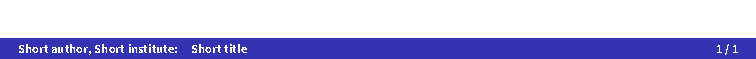
\includegraphics[page=1,width=\textwidth, trim=0 0 0 15, clip]{hackthefootline-examples}
	
	\subsection*{Two--column footline}
	"\htfconfig{%" \\
	"    title=short, authinst=onlyauthor," \\
	"    date=none, framenrs=none}" \\[\smallskipamount]
	\includegraphics[page=2,width=\textwidth, trim=0 0 0 15, clip]{hackthefootline-examples}
	
	\subsection*{Three-column footline}
	"\htfconfig{%" \\
	"    title=short, authinst=instpths," \\
	"    date=short, framenrs=fraction}" \\[\smallskipamount]
	\includegraphics[page=3,width=\textwidth, trim=0 0 0 15, clip]{hackthefootline-examples}



	\section{Examples}
	\subsection{Setting up \texttt{hackthefootline}}\label{examples-setup}
	\paragraph{Example 1:}
	"\usepackage[onecol]{hackthefootline}" \\
	\textit{Effect:} A one-column footline \\
	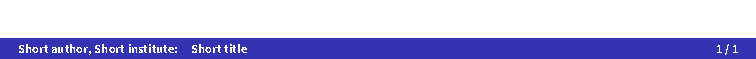
\includegraphics[page=1, width=\textwidth, trim=0 0 0 15, clip]{hackthefootline-examples}
	
	
	\paragraph{Example 2:}
	"\usepackage[twocols]{hackthefootline}" \\
	\textit{Effect:} A two-column footline \\
	\includegraphics[page=2, width=\textwidth, trim=0 0 0 15, clip]{hackthefootline-examples}
	
	\paragraph{Example 3:}
	"\usepackage[threecols]{hackthefootline}" \\
	\textit{Effect:} A three-column footline \\
	\includegraphics[page=3, width=\textwidth, trim=0 0 0 15, clip]{hackthefootline-examples}
	
	\paragraph{Example 4:}
	"\usepackage{hackthefootline}" \\
	\textit{Effect:} The footline gets removed
	
	
	\subsection{Switching templates}\label{examples-switchtemplates}
	This section assumes, that the "\usepackage[twocols]{hackthefootline}" command was used to load the "hackthefootline" package. \\[\medskipamount]
	The preamble contains the following commands for setting the information about title, author, institute and date: \\[\smallskipamount]
	"\title[Short Introduction]{%" \\
	"    A short introduction on \texttt{hackthefootline}'s facilities}" \\
	"\author[S. Friedl]{Sebastian Friedl}" \\
	"\institute[Some Institute]{Some Institute far, far away}" \\
	"\date[2018/01/15]{January 15, 2018}"
	
	\medskip
	We will start with step 1 and continue further on, each step is changing the result of the last one.
	
	\paragraph{Initial style:}~ \\
	\includegraphics[page=4, width=\textwidth, trim=0 0 0 15, clip]{hackthefootline-examples}
	
	\paragraph{Step 1:} Show fraction frame numbers \\
	\textit{Command:} "\htfconfig{framenrs=fraction}" \\
	\textit{Effect:} \\
	\includegraphics[page=5, width=\textwidth, trim=0 0 0 15, clip]{hackthefootline-examples}
	
	\paragraph{Step 2:} Show the short version of the date \\
	\textit{Command:} "\htfconfig{date=short}" \\
	\textit{Effect:} \\
	\includegraphics[page=6, width=\textwidth, trim=0 0 0 15, clip]{hackthefootline-examples}
	
	\paragraph{Step 3:} In addition to the author, show the insitute in parentheses \\
	\textit{Command:} "\htfconfig{authinst=instpths}" \\
	\textit{Effect:} \\
	\includegraphics[page=7, width=\textwidth, trim=0 0 0 15, clip]{hackthefootline-examples}
	
	\paragraph{Step 4:} Show the long, full title \\
	\textit{Command:} "\htfconfig{title=long}" \\
	\textit{Effect:} \\
	\includegraphics[page=8, width=\textwidth, trim=0 0 0 15, clip]{hackthefootline-examples}
	
	\paragraph{Step 5:} The right column is too full now. Remove the frame numbers \\
	\textit{Command:} "\htfconfig{framenrs=none}" \\
	\textit{Effect:} \\
	\includegraphics[page=9, width=\textwidth, trim=0 0 0 15, clip]{hackthefootline-examples}
	
	\paragraph{Step 6:} Switch to a one-column footline and remove the date \\
	\textit{Command:} "\htfconfig{cols=one, date=none}" \\
	\textit{Effect:} \\
	\includegraphics[page=10, width=\textwidth, trim=0 0 0 15, clip]{hackthefootline-examples}
	
	\paragraph{Step 7:} Remove the footline \\
	\textit{Command:} "\htfconfig{cols=none}" \\
	\textit{Effect:} No footline will be shown (but a space above the frame's bottom …)
\end{document}